\section{About this project} 

The ULTRACAM high speed photometry camera (hereafter, ULTRACAM) had its `first-light' at the William Herschel Telescope (WHT) on the 16 May 2002. Since then it has been used on many occasions at three telescopes, namely the William Herschel Telescope (WHT), La Palma, Islas Canarias, the Very Large Telescope (VLT), Cerro Paranal, Chile and New Technology Telescope (NTT), La Silla, Chile. The camera is portable and can travel between these telescopes. It was designed specifically to take high speed photometry of faint objects in three colours. These three attributes are fundamental to understanding the scientific value of ULTRACAM and also set important context about the reason for doing this project, so let's first discuss each one in turn. 

\emph{High-speed:} By 'high speed' we mean that ULTRACAM can take images of the telescope fields at a high frame rate. Astronomy very often relies on long exposures to capture enough light in order to perform the measurements required. The general assumption is that the objects we are looking at do not change on short timescales. This is not true for all objects. Indeed, some objects are variable on incredibly short timescales. At the most extreme end of this scale are pulsars, which spin at a rate of 100s of times per second. Binary stars that are interacting with each can show variability on the scale of \textless 2 seconds to several years. When compact objects such as White Dwarfs are eclipsed in a binary system, the light from the object can disappear in the about 2-3 minutes, making a very sharp eclipse profile. In fact, a sub-class of these stars, Cataclysmic Variables have a bright compact component called a 'hot-spot' that can disappear in a matter of seconds. The ingress and egress of exoplanets transiting the disc of their parent star can last for a few minutes or so. Certain pulsating stars show variations in their light output on timescales of a few minutes. 

\emph{Faint objects:} ULTRACAM was designed to be installed on some of the larger telescopes in the world. The WHT has a mirror diameter of 4.2 metres, NTT 3.5 metres and the VLT 8.2 metres. These large mirrors are important for gathering a great amount of light from our target objects. Since ULTRACAM is a 'high-speed' camera, we do not have the luxury of taking long exposures in order to accumulate enough light, we need our mirror to give us as many photons as possible. The combination of ULTRACAM with large telescopes like the VLT has enabled researches to take high speed photometric measurements of targets such as GU Mus, which is an 20th magnitude (now in quiescence) x-ray nova with a time resolution of $\sim 5$ seconds. It can also take even higher speed data of cataclysmic variables, such as V834Cen, a 17th magnitude polar CV at a time resolution of $\sim 0.05$ seconds.

\emph{Colour:} In Astronomy, colour is an important property that can tells a great deal about the object. By measuring the amount of light, or \emph{flux} from the object in different portions of the electromagnetic spectrum, we can deduce properties of the object, most notably, temperature. Colour is also valuable during an eclipse. If the colour of our target changes during the eclipse, this allows us to de-couple the separate colours of the two objects in the binary. During an exoplanet transit, subtle changes in colour during primary transit and also just before and after secondary transit, might help us determine the colour of the planet and therefore give us a clue to the composition of its surface and/or atmosphere. \emph{Comment: Is this really true for ULTRACAM? Or do we need more infra-red sensitive instruments... check with exoplanet guys}. 

Thanks to its design, ULTRACAM has been used primarily to study the sorts of objects listed above. In nearly all observing runs there is a specific target object defined and the camera and telescope are set up to optimise the observations for this kind of object. Exposure times, filters and field sizes are chosen to pick out the target object as cleanly as possible and provide the kind of data that the observing astronomer needs. Nevertheless, the nature of the camera means that it will also be capturing data on other objects that just happen to be in the field of view (or indeed 'passing-through' the field of view) during the run. One of the main reasons for automating the pipeline is that we might, serendipitously, discover objects that, although not the intended targets of the run, are, nevertheless, displaying some kind of variability. Depending on the size and orientation of the windows that the observer has selected and how crowded the sky in the field of view is, we could have many objects recorded in the raw data that have not had light-curves produced. Producing and analysing these new light-curves will hopefully allow us to discover new variable objects. 

\section{Candidate objects}
What kinds of objects should we expect to discover when sifting through the ULTRACAM archive? Obviously, we should expect to find variables of similar classes to those that the camera was designed to observe, but also (we hope) some that, due to the nature of the observations made, may appear in these raw data serendipitously.  In this section we list some of these object classes. 

\subsection{Eclipsing binaries}
Many of the stars in the galaxy do not exist alone in their place, but form one component of a multiple star system. It is estimated that field star population in the solar neighborhood consists of 50\% binary systems, \cite{binaryfraction}. Some of these systems have their orbit in a plane that is viewed 'side-on' from Earth ($i \sim 90^\circ$) and therefore the geometry is such that eclipses will occur at least once per orbit. These eclipses will be seen as a drop in flux. The eclipse profile will indicate the relative sizes of the two objects in the system. Also, the timing of the event gives us an indication of the separation distance. If the two objects differ in temperature, then the eclipse will show a change in colour which will be detected by ULTRACAM's 3-channel camera. Since the typical run length for ULTRACAM is about 1-3 hours, we are biased towards detecting binaries with short orbital periods (\textless 1 day). 

\subsection{{W UMa} systems}
{W UMa} systems are binary systems in which both stars have filled their Roche lobes and the stars are effectively merged, although their cores are seprate and in orbit about each other. Since their atmospheres are in contact and they are in stable orbits, we can assume that they are in thermodynamic equilibrium. As these objects rotate, we will see a change in flux due to the non-spherical shape of the system that is presenting different surface areas towards earth and possible eclipses too. The depth of this flux change will depend on the inclination of the orbit. If we are seeing the orbit 'from-above', with the inclination, $i \sim 0$ then we will see no change at all. At inclinations of $i \sim 90$ we will see the maximum drop in flux of approximately $\sim50\%$. Since these bodies are in thermodynamic equilibrium we do not expect to see a change in colour during the orbital cycle. 
{W UMa} stars are binaries where both stars are in contact with each other. Also, each star in the contact binary is significantly distorted, resulting in ellipsoidal variations of the flux due to the fact that the projected area of the stars is constantly changing. Their periods fall in the 6 to 20 hour range and should therefore be obvious in the ULTRACAM data for a run of duration 30 minutes or more. 

\emph{Comment: Need a reference for a {W UMa} review article.}

\subsection{Ellipsoidal variables}
Stars in binaries that are not in contact but still sufficiently close to each other to cause tidal distortion of one or more of the components will show variability for the same reasons as the {W UMa} stars, ie that the projected area of the star presented towards the Earth varies over the orbital cycle. The typical change in brightness of an ellipsoidal variable is about 0.1 magnitudes or a 10\% change in flux. Orbital periods should be similar to those of the {W UMa} category, about 6-20 hours. 

\subsection{Cataclysmic variables}
Cataclysmic variables are stars that are nominally in contact in that at least one of the stars has filled its Roche lobe and material is streaming from this star onto the companion. The companion in this case is a White Dwarf, that has a mass of somewhere between $0.4 M_{\odot}$ and $1.4 M_{\odot}$, yet a radius that is similar to the radius of the Earth. The White Dwarf's surface is, therefore, a long way from where this flowing material leaves the donor star and starts to fall towards the White Dwarf. Since the material has its own angular momentum, it cannot fall directly toward the White Dwarf, but spirals inward, usually forming an accretion disc through which it eventually migrates onto the White Dwarf's surface. 

Cataclysmic variables are highly variable on many different timescales. On the timescale of centuries, they can undergo \emph{nova} where they explode a shell of hydrogen that has been built up on their surface, increasing their brightness by 6-19 magnitudes. Over a period of weeks to months, their accretion disks can go into \emph{outburst}, increasing their magnitudes by a few magnitudes. On the timescale that is most relevant to a typical ULTRACAM run, we can expect to see eclipses of the white dwarf, bright-spot and disc (assuming this is an eclipsing system) and flickering caused by the accretion stream flowing onto the bright-spot. 

\emph{Comment: Reference to Coel Hellier's book here (or Brian's book). }

\subsection{Intrinsic variables}

\subsubsection{RR Lyrae stars}
RR Lyrae stars are horizontal branch stars that have evolved away from the main sequence and are in the instability strip. Pulsations in RR Lyraes are driven primarily by Helium ionisation zones in their interiors, also known as the $\kappa$ mechanism, \cite{asteroseismology}. They exhibit periods of several hours to a few days and their light curves are usually non-sinusoidal (with harmonics) and often diplay a 'sawtooth' shape. The brightness variation can be between 0.3 and 1.2 magnitudes (or 30 to 300 \%). The colours will change significantly during the cycle as the surface temperature rises and falls and this should be clear in these ULTRACAM data. 

RR Lyraes are most common in older stellar populations and it is worthwhile taking a closer look at one or two runs in the archive that were looking at the globular cluster, Omega Centaurus. 

\subsubsection{$\delta$ Scuti stars}
$\delta$ Scuti stars are driven by similar mechanisms to the RR Lyraes but are generally more massive stars and are still in the main sequence. They also exhibit non-radial pulsation modes and therefore have a shorter characteristic periods but with lower amplitudes. Typical periods for $\delta$ Scutis are from 1 hour to 7 hours, with amplitudes of around $\sim 0.1 mag$. Like the RR Lyraes the surface temperature of the star will change during the pulsation cycle and we therefore expect to see a colour modulation in the light-curve. 

\subsubsection{Pulsating White Dwarfs}
White Dwarf stars pass through a region of the HR diagram that can be seen as an extension of the classical instability strip. In these regions, the White Dwarf will experience a similar driving mechanism to that which drives pulsations for the Main Sequence and Horizontal Branch stars, namely the $\kappa$ mechanism in the White Dwarfs thin Hydrogen or Helium atmosphere. Pulsating Hydrogen White Dwarfs are known as {DAVs} or {ZZ Ceti} stars and Helium White Dwarfs as {DBV}s. Usually they have a fairly complex oscillation, with many frequencies, as they oscillate with many modes excited. Nevertheless, a pulsating White Dwarf should be fairly obvious when observed with ULTRACAM. The oscillations will have periods of a few minutes and amplitudes on the order of 0.1 magnitudes. 

\subsection{Flare stars}
Flare stars are usually red dwarf or brown dwarf stars that undergo flares in their atmospheres resulting in rapid changes in brightness on timescales of minutes to hours. Typical flare rates for {UV Cet} are about every 2.5 to 6 hours. In the optical spectrum we expect the flares to appear as impulse rises with an exponential decay lasting minutes to hours. During the flare, we can expect the intensity to double \cite{stellaractivity}. This obvious change in brightness should be detected during an ULTRACAM run. 

\subsection{Asteroids}
Solar System objects such as asteroids and Kuiper belt objects should be visible in the ULTRACAM archive. Main asteroid belt and near-Earth objects are likely to move across the field at a few arc seconds per minute, meaning that they would cover a fair fraction of the exposed CCD image during the course of a 1-2 hour run of the ULTRACAM. We can expect a $\sim 300 metre$ sized near Earth object to have a magnitude in V of around 15, \cite{neosmalltelescope} which is an appropriate level for most ULTRACAM observations. 

Kuiper belt objects will have apparent magnitudes of around $V\sim 20$ and would move only a few arcseconds per hour. It is fairly unlikely (although not impossible) that we might record one of these objects in an ULTRACAM run. 

\section{The ULTRACAM instrument} 

\subsection{Camera Optics}

The camera has three CCD detectors enabling it to capture data in three colour bands simultaneously. Two dichroic beamsplitters divide the light from the collimator into three beams, which shall hereafter be referred to as the `red', `green' and `blue' channels. The three CCD detectors are mounted at right angles to each other on the camera. Therefore, each detector is at the end of a slightly different optical path. The images produced on each of the three CCDs chips are therefore of the same field but with very slightly different orientations, distortions and offsets. Towards the edges of the chips, these differentials can add up to be on the order of 10 pixels from channel to channel. 

While the exposure timing is synchronised across the detectors, it is, however, possible to have the detector in the blue channel remain exposed and not 'read-out' while the other two are going through multiple exposures and 'read-outs'. This is to allow for longer exposures where there might be less flux in blue. Reduced flux in blue is caused by several factors, including lower transmission of the optics and atmosphere to blue light, the reduced sensitivity of the CCD detector to blue light and the intrinsic flux of most astronomical objects is lower in this channel.

\begin{figure}[!h]
\centering
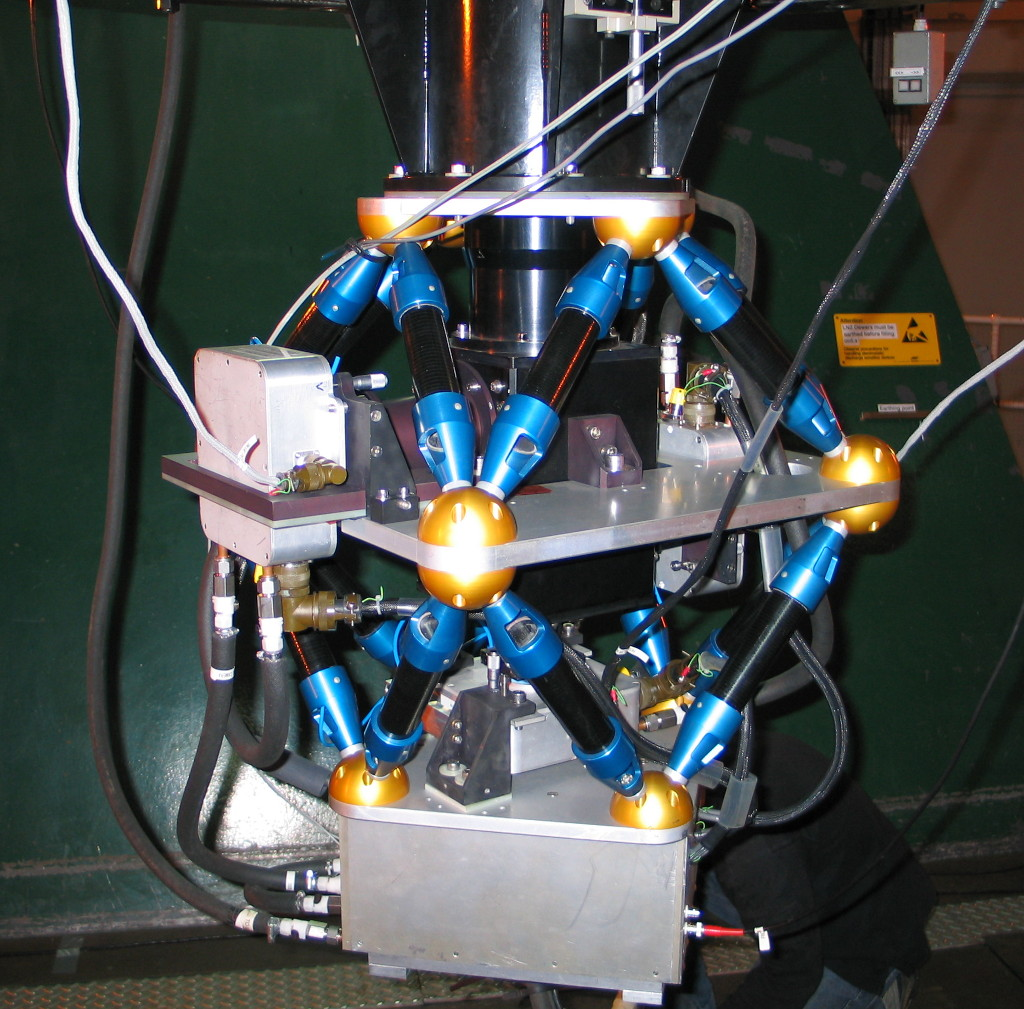
\includegraphics[width=90mm]{images/IMG_0121_scaled.JPG}
\caption{The Ultracam being commissioned in May 2002.}
\label{fig1}
\end{figure}

\subsection{Filter sets}
The filters for each channel can be altered by the observer. In usual configurations, the SDSS filters (u, g, r, i, z) are used, but there are a selection of narrow-band filters that can be substituted. Depending on the scientific measurements that the observer is trying to perform, these filters will be changed.   

\subsection{Field size and pixel scale}
ULTRACAM is usually mounted on one of the three telescopes mentioned in the introduction of this chapter (VLT, NTT, WHT). Field sizes, pixel scales and orientations are summarised in table \ref{tab:pixelscale}. The orientations quoted refer to when the camera is \emph{not} rotated. 

\begin{center}
\begin{table}
	\begin{tabular}{|l|r|r|r|}
    	\hline
		Telescope & Field size (arc minutes) & Pixel scale (arc seconds/pixel) & Orientation \\
		\hline
		WHT & 6.0x6.0 &  0.35 & N(up), E(left)\\
		NTT & 6.0x6.0 & 0.35 & N(up), W(left)\\
		VLT & 2.5x2.5 & 0.15 & N(up), E(left) \\
		\hline
	\end{tabular}
	\caption{The field sizes and pixel scales of ULTRACAM on each of the three telescopes. \emph{Comment: Confirm these figures with Tom/Elme.}}
	\label{tab:pixelscale}
\end{table}
\end{center}



\subsection{High speed operation}
A key aspect of the design of the camera is its ability to perform at high cadence, or frames per second. It is possible to have the camera read-out at up to 500Hz (frames per channel per second) \cite{dhillon07}. This makes the camera useful for observations of rapid transient events with accurate timing. Although the camera is not often used in this very high speed mode, there are a few observing runs where the camera has been operating with exposure times of approximately 0.005 seconds. These runs are described in chapter~\ref{chap:results}.

Each CCD has a total pixel area of 2057x1024 pixels. Half of these pixels are masked and never exposed to light. They are used as a temporary buffer for reading out the chip. CCD detectors are read out serially, but in order to decrease the time between exposures, the full image can be moved to the blanked-out area of the chip and this can then be read out while the un-masked area of the chip is once again exposed to light. 

\begin{figure}[!h]
\centering
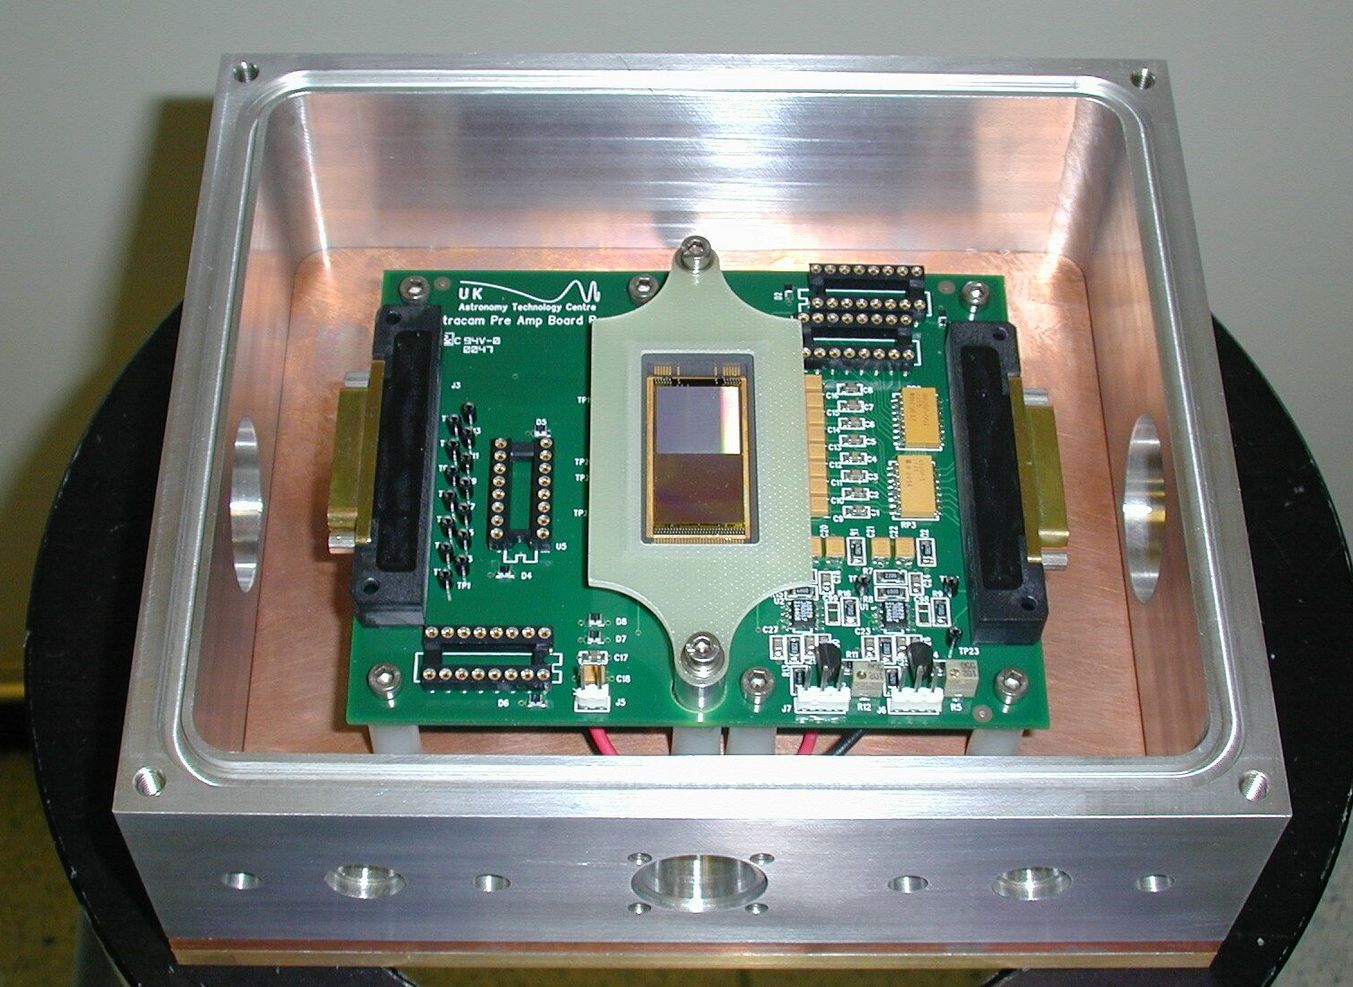
\includegraphics[width=90mm]{images/ccd.png}
\caption{One of the three CCD detectors. The masked-off area is visible in the lower half of the chip surface.}
\label{fig2}
\end{figure}

ULTRACAM gives the observer the option to reduce the area of the detector that is used for the exposure. This reduces the chip readout time and enables the higher cadences. Reducing the number of pixels exposed also decreases the amount of data storage needed for the run. The observer can define pairs of \emph{windows} that are centred on the objects of interest, or \emph{target} objects. By making the windows suitably small, the observer can use the camera in extremely high cadence mode. 

The highest cadence mode is called \emph{Drift mode}. This mode uses the masked area of the CCD chip to store several exposures simultaneously. Only the portion of the CCD that has been selected by the observer is shifted into the masked area of the CCD. The fact that the camera is not shifting the whole field of view means that the unmasked area is ready to be re-exposed almost immediately. This mode requires that only the lower portion of the detector, close to the boundary of the masked and un-masked areas, is selected by the observer. Due to the geometry of this readout mode, it is necessary that the exposed area of the CCD is immediately adjacent to the boundary with the masked-off section of the chip. This means that the camera will have to be rotated so that the target object (and a suitable comparison star) are positioned correctly. The ULTRACAM is therefore designed to be rotated about the optical axis of the telescope so that there is another degree of freedom in positioning of the target objects. For any particular run, it is possible that we can have \emph{any} orientation ($0-180^{\circ}$) of the camera relative to the sky coordinates. The ULTRACAM logs do not record this rotation angle. This is an important factor to remember when we try to find astrometric solutions for the runs.    

\begin{figure}
  \centering
  \setlength{\fboxsep}{0pt}
  \setlength{\fboxrule}{1pt}
  \fbox{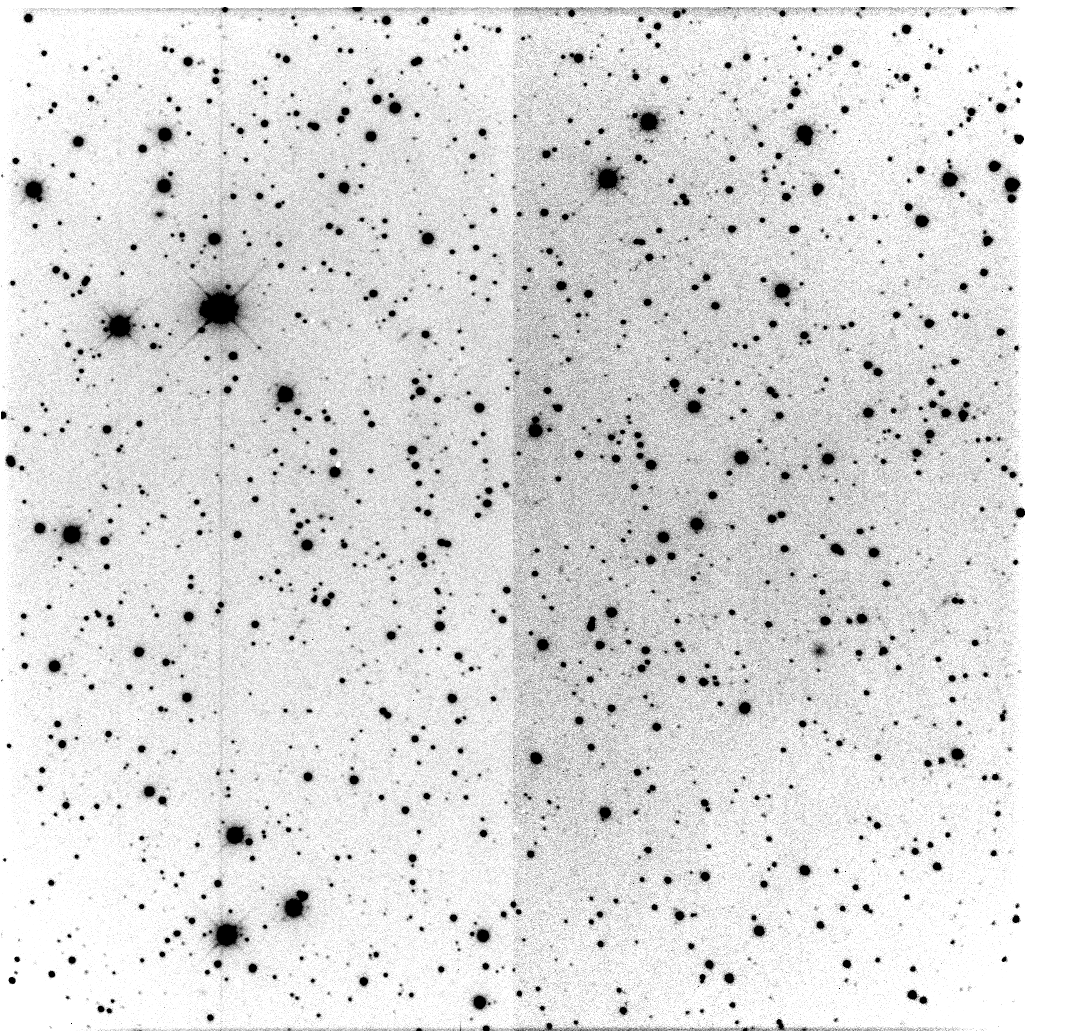
\includegraphics[width=120mm]{images/run010_r_inverted.png}}
  \caption{A 'fully' exposed CCD with 1 pair of windows (512x1024 pixels each).  This mode reads out the full area of the CCD chip, resulting in larger data size and a longer readout time. The field of view is approximately 7x7 arc minutes, but varies according to the telescope that the camera is mounted on.}
  \label{fig:KOI-824}
\end{figure}

\begin{figure}  
  \centering
  \setlength{\fboxsep}{0pt}
  \setlength{\fboxrule}{1pt}
  \fbox{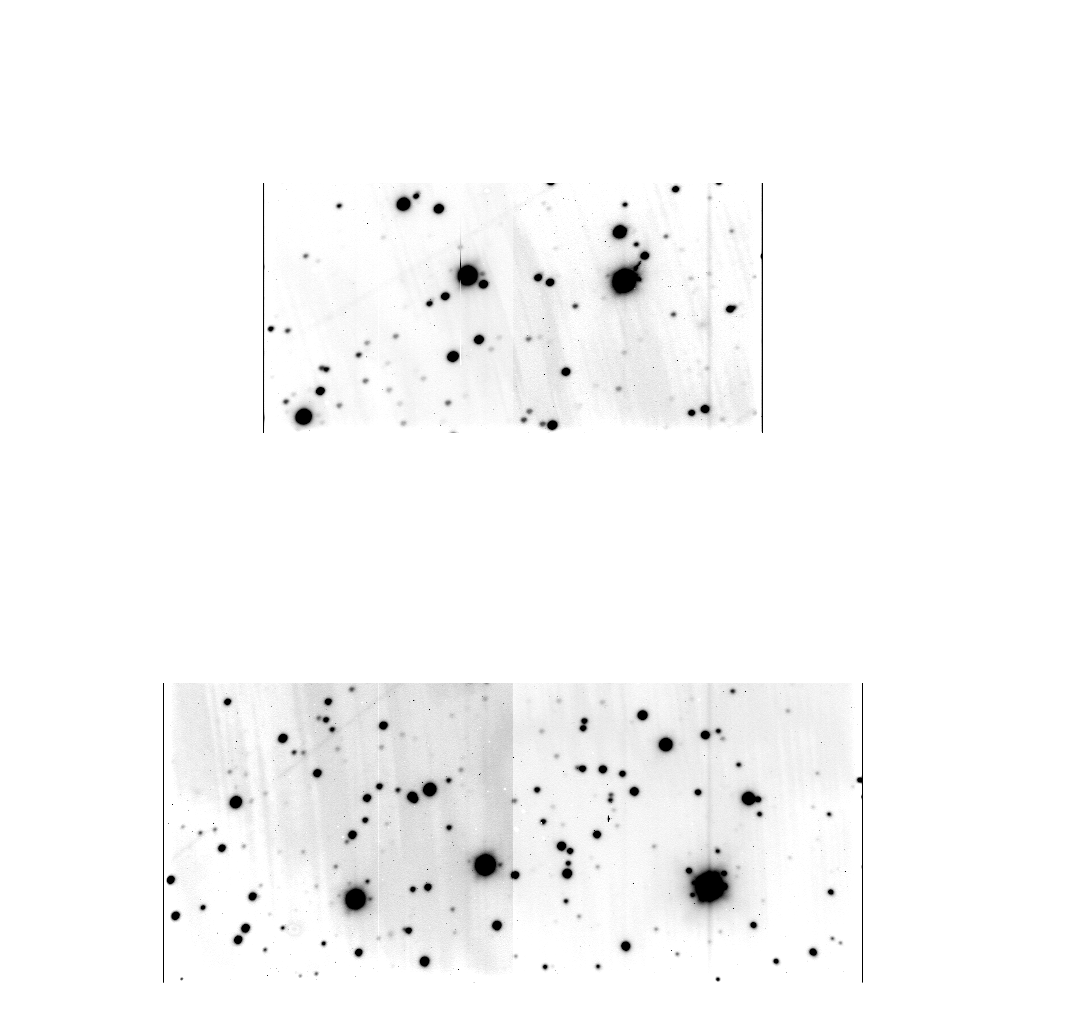
\includegraphics[width=120mm]{images/run016_r_inverted.png}}
  \caption{A 'masked' exposure with 2 pairs of windows (350x300 and 250x250 pixels each, respectively)}
  \label{fig:V713Cep}
\end{figure}

\begin{figure}  
  \centering
  \setlength{\fboxsep}{0pt}
  \setlength{\fboxrule}{1pt}
  \fbox{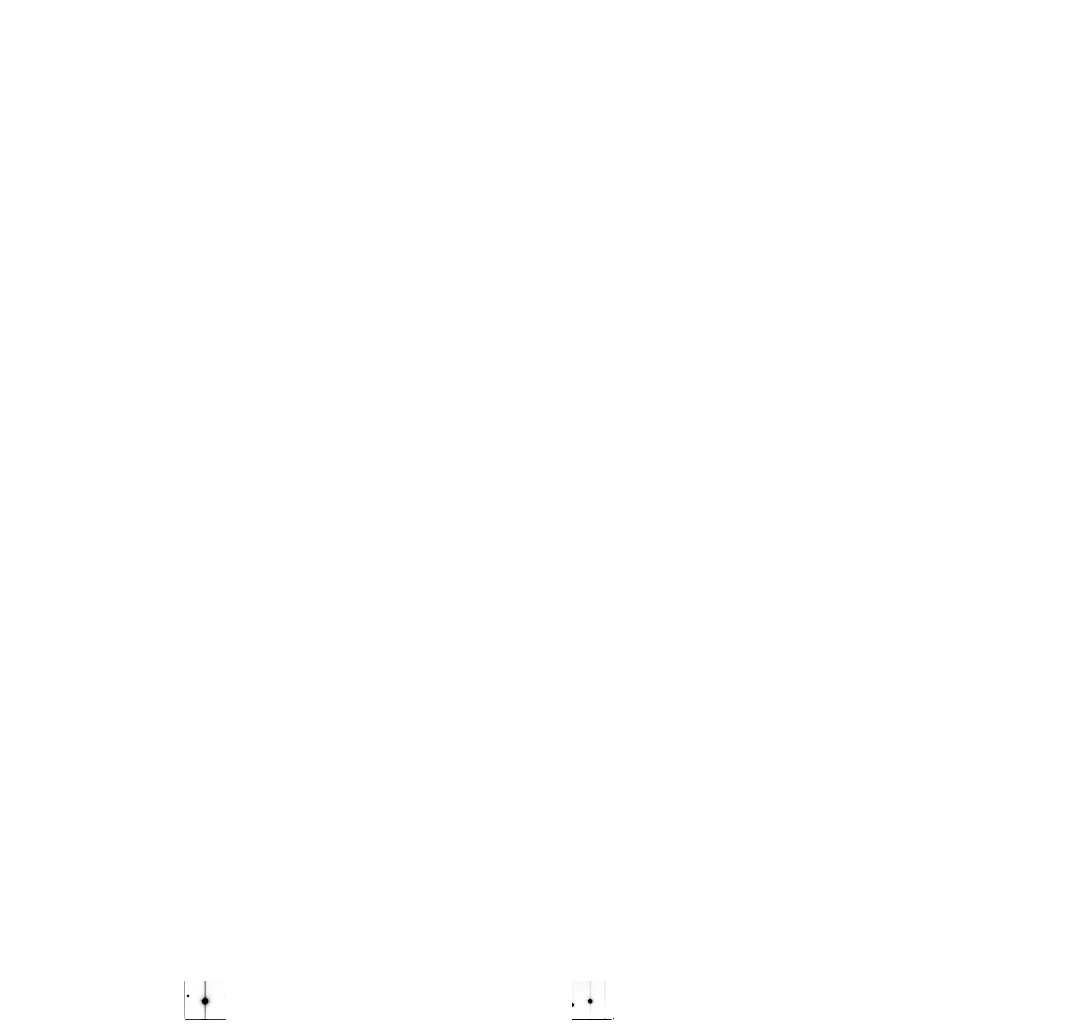
\includegraphics[width=120mm]{images/run018_r_inverted.png}}
  \caption{The camera operating in \emph{drift-mode}. Note the very small windows (172x156 pixels) located at the bottom of the imaging area.}
  \label{fig:V834Cen}
\end{figure}

More details on the camera design and operation can be found in \cite{dhillon07}.

\section{ULTRACAM data}

\subsection{Data capture}
Usually the camera remains installed on the telescope for a week or so and is used for observations on consecutive nights. Each separate recording of data is called a \emph{run}. On most nights, many \emph{runs} are recorded. A \emph{run} can be defined as a period when the camera is active and gathering data. Not all runs are used for gathering \emph{scientific} data. Some runs are used for target acquisition and camera calibration purposes. 

The types of runs are: 
\begin{itemize}
	\item \emph{Science run}: These are the runs that contain the valuable scientific data. They usually comprise the longest portions of the observations during the night, unless the camera is having difficulties or adverse conditions are preventing useful astronomical observations.
	\item \emph{Acquisition run}: These are runs, usually of short duration (ie a few minutes) during which the telescope is being moved in order to place the candidate object(s) in the field of view. The camera may also be rotated in order to align the CCD such that the targets avoid `bad' pixels or are near to the lower boundary of the detector (eg for high speed readout in Drift mode). 
	\item \emph{Flat field}: At the start and the end of the night (usually during twilight) the observer will take a few runs to create \emph{sky-flats} that will be used later for calibrating the variations in pixel sensitivity across each of the detectors.  Sky-flats are generated by exposing the camera to patches of sky during the twilight. 
	\item \emph{Bias}: A short run to build calibration readings for measuring the bias of the detector. This bias will be subtracted from these data during the reduction. 
	\item \emph{Timing calibration run}: One way to check the timing calibration of the camera is to take frames of a well-known, rapidly oscillating source, for example, the Crab Pulsar (PSR B0531+21). The timing of the optical pulses as measured by the camera can then be compared to the expected times for the pulsar. This is used as a standard clock for timing calibration.
\end{itemize}

\subsection{Typical run length}
Since ULTRACAM is designed for high-speed photometry, observers using the instrument are typically looking for variations that are clearly noticeable on timescales from a few minutes to a few hours. Most science runs last for a few hours at the most. The longest runs are usually observations of exoplanet transits which can last from about 4-7 hours. Very often, these have a break in the middle if the telescope goes through the zenith. Alt-az designs cannot always observe directly at the zenith and the run is interrupted for 3 minutes or so, while the telescope is repositioned after the zenith 'blind-spot'.

A look at the distribution of run length shows a large bulk of the runs are shorter than 5 minutes. This is because there are far more acquisition runs, flat-fields and bias runs than there are science runs. There are also many runs that are nominally science runs (and can be used as such) but are short because the observer has noticed something that they would like to change. This could be a change in focus, binning factor or integration time. The run is then cut short and a new run is started. The longest run length in the 10 year data archive is 566 minutes or 9.5 hours, taken on 25th of April 2010 at the NTT. This was for the observation of a transit of the exoplanet Wasp-15b. The output for this run can be seen at \small \url{http://deneb.astro.warwick.ac.uk/phrnaw/sitedev/2010-04-25/run020.html}. 

\begin{figure}[!h]
  \centering
  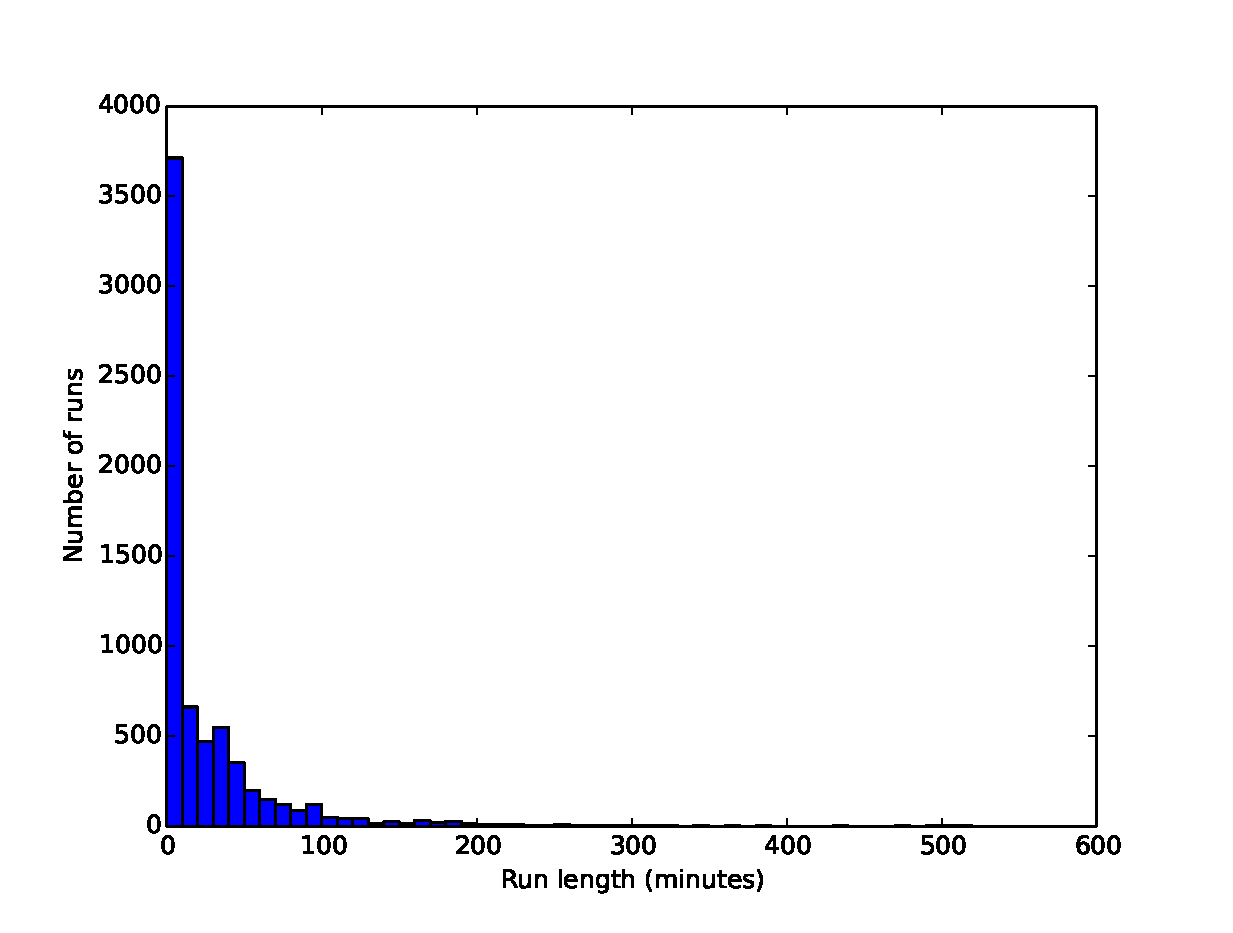
\includegraphics[width=120mm]{images/hist0-600.eps}
  \caption{Distribution of run length. Many runs are shorter than 5 minutes, but these are not usually \emph{science runs}.}
  \label{fig:histogram0-600}
\end{figure}

\begin{figure}[!h]
  \centering
  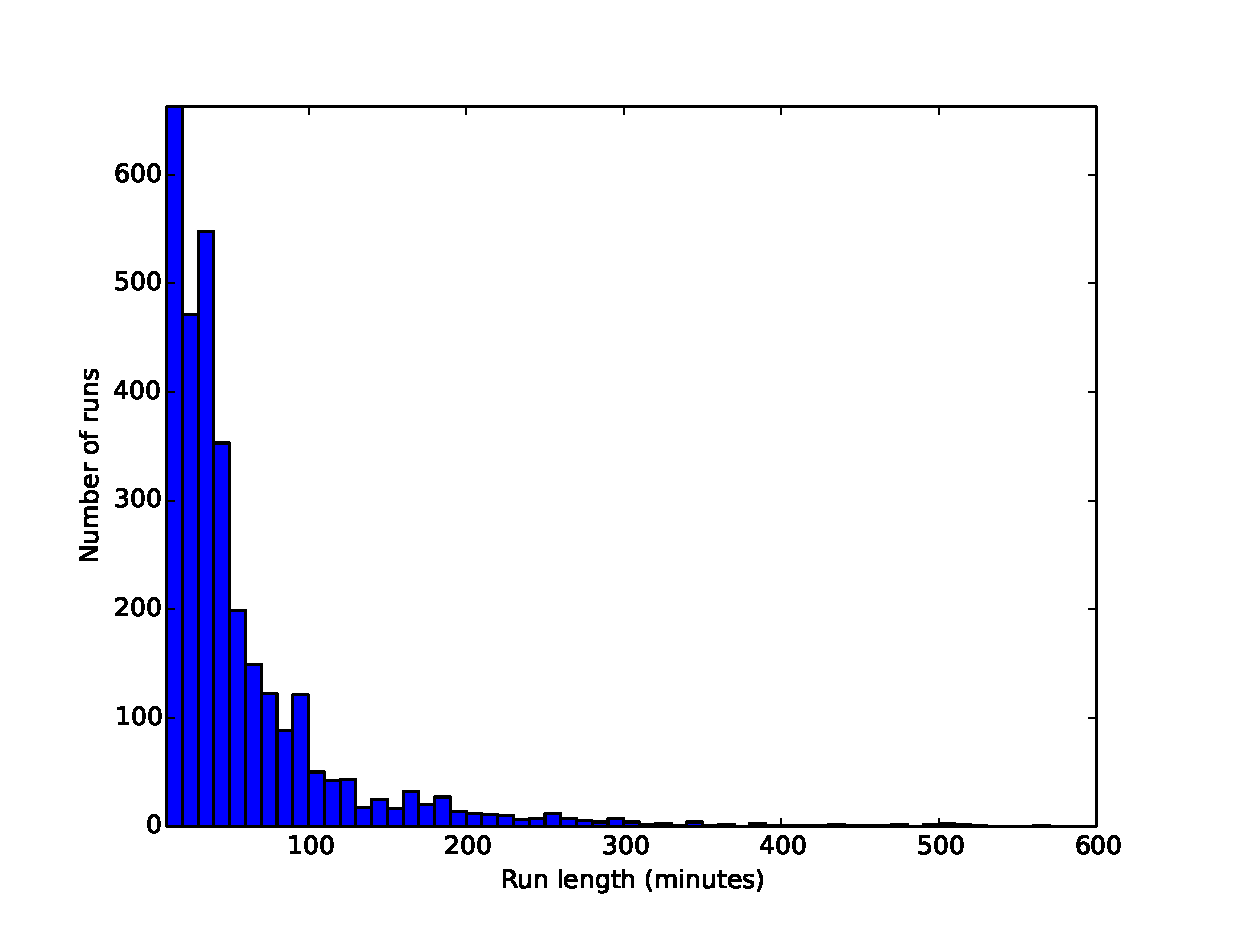
\includegraphics[width=120mm]{images/hist10-600.eps}
  \caption{Distribution of run length after removing runs shorter than 10 minutes.}
  \label{fig:histogram10-600}
\end{figure}

\begin{figure}[!h]
  \centering
  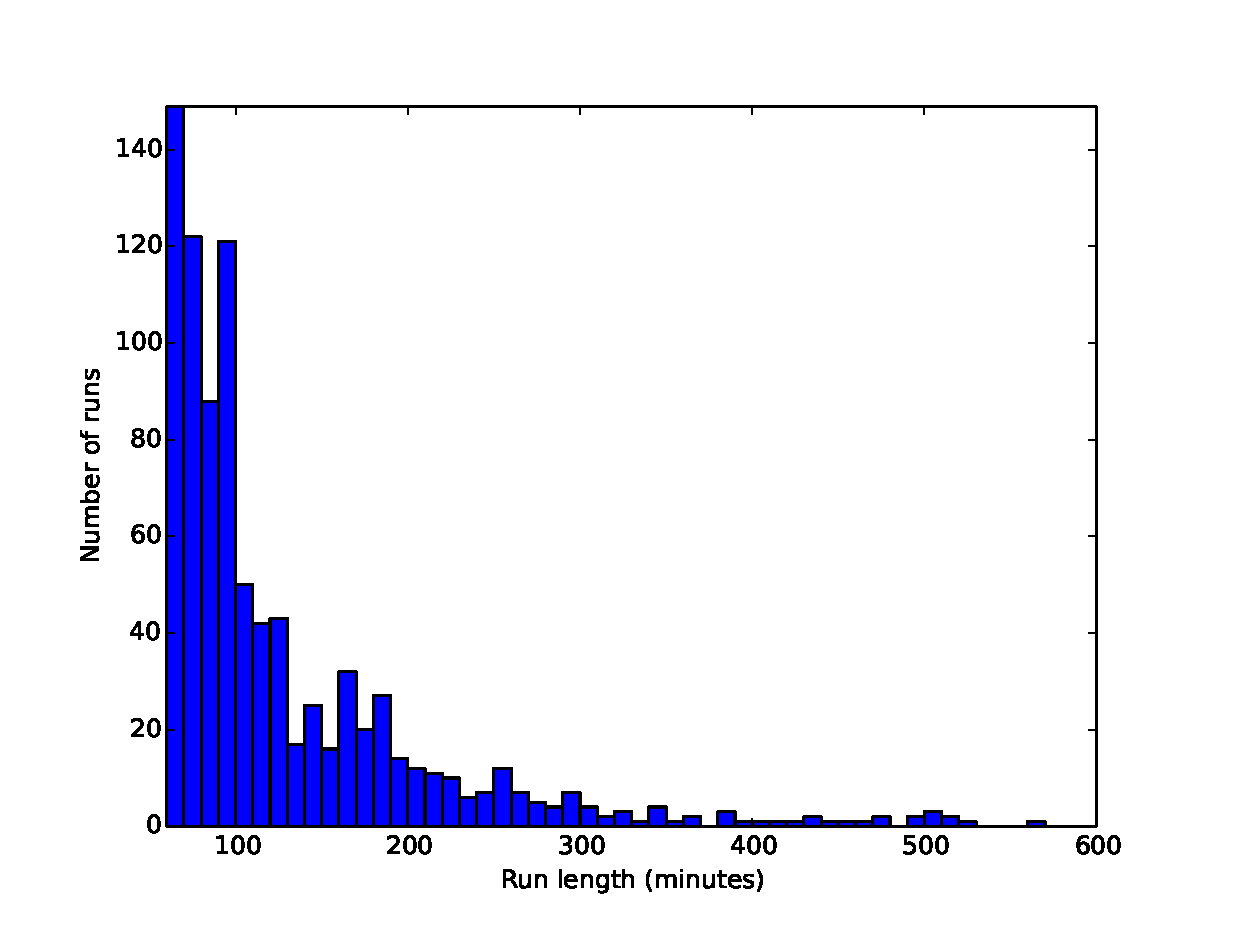
\includegraphics[width=120mm]{images/hist60-600.eps}
  \caption{Distribution of run length after removing runs shorter than 60 minutes.}
  \label{fig:histogram60-600}
\end{figure}


\begin{figure}[!h]
  \centering
  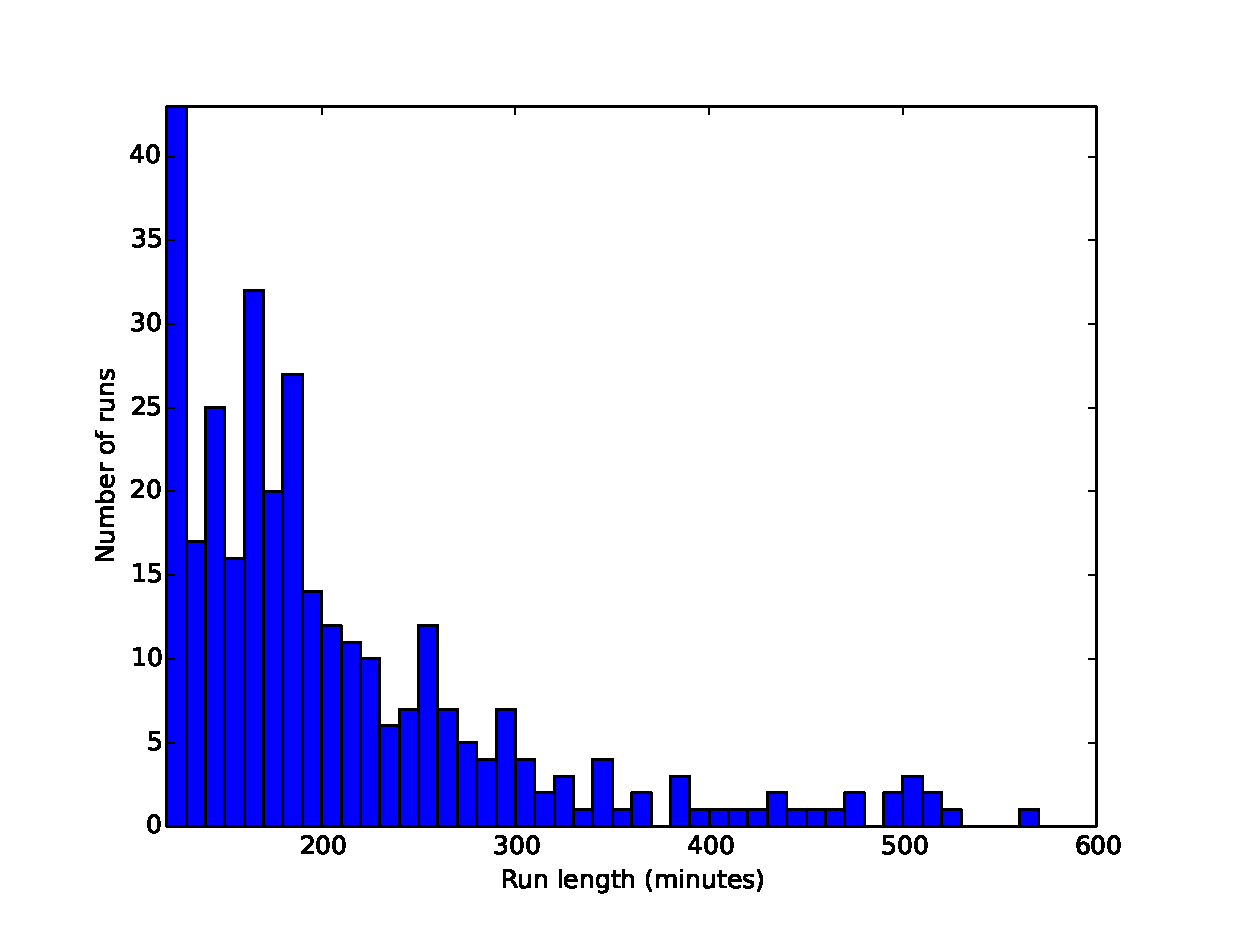
\includegraphics[width=120mm]{images/hist120-600.eps}
  \caption{Distribution of run length after removing runs shorter than 120 minutes.}
  \label{fig:histogram120-600}
\end{figure}

\subsection{Run cadences}
As mentioned in the section describing the camera, ULTRACAM was designed specifically for high-speed photometry. Certain phenomena in astrophysics have observable variability in the optical region of the spectrum that is apparent over relatively short periods. Ultra-compact binaries, Cataclysmic variables, Neutron stars, etc all have signals that can be resolved at even sub-second intervals. ULTRACAM is also mounted on some relatively large telescopes, with mirrors ranging from $4.2m - 8.2m$ in diameter. This means that it is able to perform high-speed photometry of relatively faint objects. Since the commissioning of the camera in 2002, it has been used to observe a variety of objects, summarised in table \ref{tab:breakdown}. 

Only certain objects require the highest cadences (\textless 1 second). These are X-ray binaries, Polars, Pulsars, Flare stars. Many other science runs can use the camera with a \textgreater 1 second exposure time. Long runs for exoplanet transit observations often use longer exposures of 2-3 seconds. The longest exposure times are around 20-25 seconds. This is only required when the object being observed is extremely faint.  

\begin{table}
  \begin{center}
	\begin{tabular}{|l|r|}
		\hline
		Target & Time (percent) \\
		\hline
		Cataclysmic Variables & 25.3 \\
		X-ray binaries & 17.4 \\
		sdB stars/asteroseismology & 11.2 \\
		etc & x.y \\
		\hline
	\end{tabular}
  \end{center}
\label{tab:breakdown}
\caption{Breakdown of how ULTRACAM is used. \emph{Comment: This is the out of date table from \cite{dhillon07}. Should update this.}}
\end{table}


\begin{figure}[!h]
  \centering
  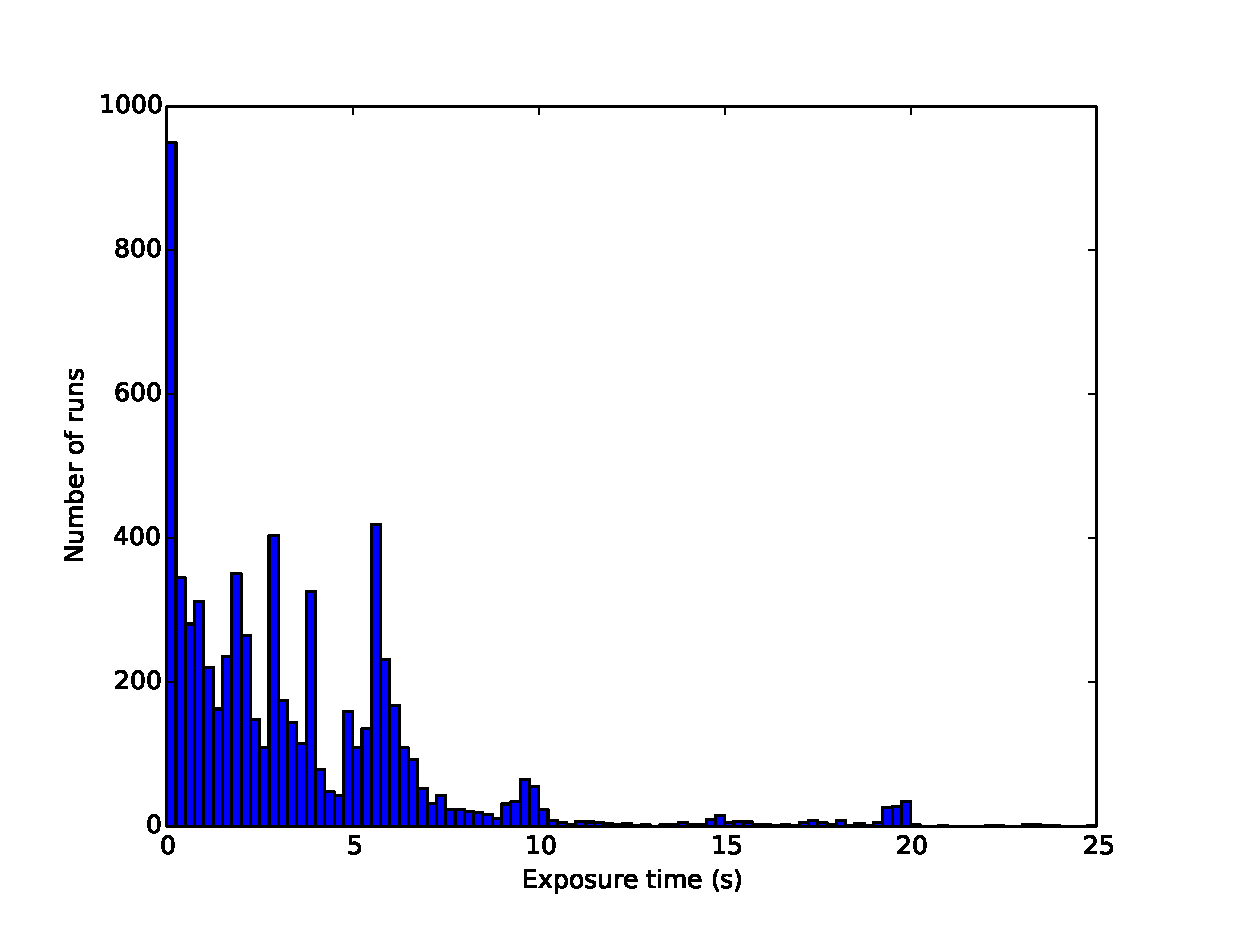
\includegraphics[width=120mm]{images/cadences_hist0-25.eps}
  \caption{Distribution of exposure times used in the \emph{science} runs.}
  \label{fig:cadences}
\end{figure}

Figure \ref{fig:cadences} shows a distribution of exposure times by run, for all of the \emph{science} runs in the ULTRACAM data archive. There are several groupings apparent in the histogram. Firstly, the very short exposures for the rapidly variable objects, such as Polars, Pulsars and X-ray binaries. Then there is a cluster of runs with exposure times of 2, 3, 4 and 5.5 seconds. These are typically observations of eclipsing binaries. The next cluster occurs at about 10 seconds, which are usually runs for exoplanet transits. The final cluster of run lengths occurs at around 20 seconds, usually reserved for very faint objects, $V\sim 20$.

\begin{table}
  \begin{center}
	\begin{tabular}{|l|r|}
		\hline
		Exposure time (seconds) & typical target \\
		\hline
		0-1 second & X-ray binaries, polars, CVs \\
		2, 3, 4, 5.5 seconds & eclipsing binaries, exoplanet transits \\
		10 seconds & exoplanet transits \\
		25 seconds & faint objects \\
		\hline
	\end{tabular}
  \end{center}
\label{tab:breakdown}
\caption{Typical exposure times and the type of target being observed. Comment: Characterisation here is not thorough. Will clean it up if this table is valuable.
}
\end{table}

\subsection{The data archive}
At the time of writing, the ULTRACAM data archive comprises of about 10 terabytes. This can be broken down as:
\begin{itemize}
	\item \emph{406} nights on which ULTRACAM was operational at a telescope.
	\item \emph{12 649} runs, including science runs, acquisition runs, flat fields and biases. 
	\item \emph{119 817 742} frames in total. This total includes all the frames for each channel: red, green and blue.
	\item \emph{10 542 378 791 454} bytes or 10.54 terabytes of raw image data.
\end{itemize} 

The data set is relatively large and is housed on a network-mounted storage device that is only available through the internal university computer network. This means that it is not possible to access these data from remote locations (for example, by research collaborators in different institutions). If a researcher needs to access the output of an observing run, then they need to contact a member of department at Warwick or Sheffield and request a data reduction. There is no means of accessing or exploring the ULTRACAM data set from a remote location. Providing a simple means of accessing these data from remote locations would benefit all of the research collaborators and is one of the aims of this project.


